\documentclass{article}
\usepackage{amsmath,amsthm,amsfonts,microtype,amssymb}
\usepackage{enumitem}
\usepackage{parskip}
\usepackage{mathpazo}
\usepackage{tikz-cd}
\usepackage{geometry}
    \geometry{top=1in}
\usepackage{float}
\usepackage{graphicx}    

\usepackage{hyperref}
    \hypersetup{%
        colorlinks=true,
        linkcolor=blue,
        filecolor=blue,      
        urlcolor=blue,
        bookmarks=true,
        pdfpagemode=FullScreen,
    }


\title{Homework 05 \\ Galois Correspondence of Covering Space}
\author{Algebraic Topology - Winter 2021}
\date{Due: \textbf{March 04, 2021, 11:59 pm}}

\begin{document}
\pagenumbering{gobble}
\maketitle

For this problem set assume that all the spaces are \textit{nice}.
\begin{enumerate}
\item 
  Consider the following commuting diagram
  \begin{center}
    \begin{tikzcd}
      X \arrow[dr, "\ell_3", swap] \arrow[rr, "\ell_1"]
      && Z \arrow[dl, "\ell_2"]\\
      & Y.
    \end{tikzcd}
  \end{center}
  \begin{enumerate}
  \item Show that if $\ell_2$ and $\ell_3$ are covering maps then so is $\ell_1$. 
  \item Find some conditions under which if $\ell_1$ and $\ell_2$ are covering
    maps then so is $\ell_3$. Why does the \textit{natural} proof not work for all  $\ell_1$ and $\ell_2$.
  \end{enumerate}
\item 
  \begin{enumerate}
  \item Construct a covering map from a torus to a Klein bottle.
    \begin{figure*}[h]
      \centering
      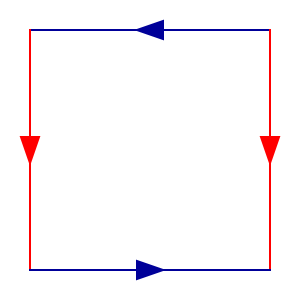
\includegraphics[width=75]{images/klein-bottle.png} 
      \label{fig:klein_bottle}
    \end{figure*}
  \item Classify all the connected covers, up to isomorphism, of the Klein bottle.
  \end{enumerate}
\item problem about free groups and covers of $S^1 \vee S^1$. 
  test
\end{enumerate}


\section*{Suggested exercises for practice from Hatcher}

\begin{description}
    \item[Pg. 38] 5, 6, 7
    \item[Pg. 39] 16, 17
\end{description}

\end{document}
